\documentclass[aip,jmp,reprint,amsmath,amssymb]{revtex4-2}

\usepackage{bm}
\usepackage{graphicx}

\newtheorem{theorem}{Theorem}
\newtheorem{lemma}{Lemma}
\newcommand{\D}{\mathcal{D}}
\newcommand{\E}{\mathbb{E}}
\newcommand{\Tr}{\operatorname{Tr}}
\newcommand{\id}{\operatorname{id}}
\newcommand{\eps}{\epsilon}
\newcommand{\CE}{C_{\mathrm E}}
\newcommand{\ketbra}[2]{|#1\rangle\!\langle#2|}

\begin{document}

\title{Directional stability of the reverse-depolarizing entanglement-assistance benchmark for qubit entanglement-breaking channels}

\author{Xiaojian Zeng}
\email{xiaojianzeng@foxmail.com}
\affiliation{PBC School of Finance, Tsinghua University, 100190, China}

\date{September 13, 2026}

\begin{abstract}
Entanglement-breaking channels destroy entanglement transmitted through them, yet preshared entanglement can still enhance their classical communication rates.  The reverse-depolarizing qubit channel realizes the enhancement factor $K_*=5.079759\ldots$ and is a sharp endpoint within the unital qubit class.  We determine the one-sided behavior along every fixed entanglement-breaking ray from this endpoint.  For $\Phi_\eps=(1-\eps)\mathcal D+\eps\Psi$, let $c_\Psi$ be the overlap of the normalized Choi state of $\Psi$ with the maximally entangled state.  If $c_\Psi>0$, the capacity gap $K_*C(\Phi_\eps)-C_{\mathrm E}(\Phi_\eps)$ equals $c_\Psi\eps\log_2(1/\eps)+O_\Psi(\eps)$.  If $c_\Psi=0$, the perturbation lies on a unital Pauli face and the gap is linear, with an explicit coefficient fixed by its largest contraction eigenvalue.  Consequently every fixed nonconstant entanglement-breaking ray moves strictly below the endpoint factor for sufficiently small positive $\eps$.  The proof controls the full input and ensemble optimizations.  The result is directional: it gives neither a uniform neighborhood nor a solution of the comparison over all qubit entanglement-breaking channels.
\end{abstract}

\maketitle

\section{Introduction}

Preshared entanglement changes the classical communication capability of a noisy quantum channel even when the channel itself cannot preserve entanglement; early work obtained exact enhancements for selected noisy channels.\cite{Bennett1999}  The entanglement-assisted classical capacity $\CE$ has a single-letter mutual-information formula,\cite{Bennett2002,Holevo2002} whereas the unassisted classical capacity generally involves regularization.  For an entanglement-breaking (EB) channel, however, additivity of the Holevo information gives $C=\chi$.\cite{Shor2002}  The ratio $\CE/C$ is therefore an especially direct measure of the value of preshared entanglement in this class.

For the qubit depolarizing family, Holevo identified the reverse-depolarizing completely positive endpoint and obtained the ratio\cite{Holevo2002}
\begin{equation}
 K_* = \frac{2-\log_2 3}{1-h_2(2/3)}
      = 5.079759330211\ldots,
 \label{eq:Kstar}
\end{equation}
where $h_2(x)=-x\log_2x-(1-x)\log_2(1-x)$.  A sharp bound with this factor is known for all unital qubit channels,\cite{Belzig2023} while a later theorem bounds the enhancement for every finite-dimensional channel with a dimension-dependent constant.\cite{Wolff2025}  The nonunital EB sector is not reduced to a Pauli channel by input and output rotations, so the unital argument does not control perturbations that translate the Bloch ball.

Here we establish a local, fixed-direction statement at the reverse-depolarizing endpoint.  Generic EB perturbations fill the one-dimensional kernel of its Choi state.  This creates an $\eps\log(1/\eps)$ entropy term in the joint reference--output state, while all single-system outputs remain uniformly full rank and their Holevo information changes only linearly.  Perturbations that do not fill the kernel form a special unital face; on that face the deficit is instead linear.  The optimizer of $\CE$ is allowed to move, and the ensemble in $\chi$ is unrestricted throughout.

The conclusion is deliberately narrower than a neighborhood theorem.  The perturbing channel $\Psi$ is fixed before $\eps\downarrow0$, and both the remainder and the threshold for strictness may depend on $\Psi$.  Directions $\Psi=\Psi(\eps)$ are outside the result, as is the global comparison over all qubit EB channels.

\section{Channels, capacities, and the main result}
\label{sec:model}

All Hilbert spaces are two dimensional, logarithms are base two, and rates are in bits per independent channel use.  We use the input-first, unnormalized Choi matrix
\begin{equation}
 J_\Phi=\sum_{i,j=0}^{1}\ketbra{i}{j}\otimes\Phi(\ketbra{i}{j}),
 \qquad \Tr_BJ_\Phi=I.
 \label{eq:choi}
\end{equation}
Thus $J_\Phi/2$ is a state.  A qubit channel is EB exactly when this Choi state is separable; equivalently in $2\otimes2$, its partial transpose is positive.\cite{Horodecki2003,Ruskai2003}

For an ensemble $\{p_x,\rho_x\}$, define
\begin{equation}
 \chi(\Phi)=\sup_{\{p_x,\rho_x\}}
 \left[S\!\left(\Phi(\bar\rho)\right)
 -\sum_xp_xS\!\left(\Phi(\rho_x)\right)\right],
 \quad \bar\rho=\sum_xp_x\rho_x,
 \label{eq:holevo}
\end{equation}
and
\begin{equation}
 \CE(\Phi)=\max_\rho I(\rho,\Phi),\qquad
 I(\rho,\Phi)=S(\rho)+S(\Phi(\rho))-S(W_{\rho,\Phi}),
 \label{eq:ce}
\end{equation}
where $W_{\rho,\Phi}=(\id\otimes\Phi)(\ketbra{\psi_\rho}{\psi_\rho})$ for any purification of $\rho$.  For EB channels, $C(\Phi)=\chi(\Phi)$.\cite{Shor2002}

Let
\begin{equation}
 \D(\rho)=\frac{X\rho X+Y\rho Y+Z\rho Z}{3}.
 \label{eq:D}
\end{equation}
It acts on Bloch vectors as $\bm r\mapsto-\bm r/3$ and is the $p=4/3$ endpoint of $\D_p(\rho)=(1-p)\rho+pI/2$.  With $|\Omega\rangle=(|00\rangle+|11\rangle)/\sqrt2$,
\begin{equation}
 \frac{J_\D}{2}=\frac{I_4-\ketbra{\Omega}{\Omega}}{3},\quad
 \chi(\D)=1-h_2(2/3),\quad
 \CE(\D)=2-\log_2 3.
 \label{eq:endpoint}
\end{equation}

Fix a qubit EB channel $\Psi$ and form the EB ray
\begin{equation}
 \Phi_\eps=(1-\eps)\D+\eps\Psi,\qquad 0\leq\eps\leq1.
 \label{eq:ray}
\end{equation}
Writing the Bloch action of $\Psi$ as $\bm r\mapsto\bm t_\Psi+T_\Psi\bm r$, set
\begin{equation}
 c_\Psi=\langle\Omega|J_\Psi/2|\Omega\rangle
 =\frac{1+\Tr T_\Psi}{4},\qquad
 G(\Phi)=K_*\chi(\Phi)-\CE(\Phi).
 \label{eq:candG}
\end{equation}

\begin{theorem}[Fixed-ray two-regime asymptotic]
\label{thm:main}
For every fixed qubit EB channel $\Psi$, as $\eps\downarrow0$:
\begin{enumerate}
 \item If $c_\Psi>0$, then
 \begin{align}
  \CE(\Phi_\eps)&=\CE(\D)-c_\Psi\eps\log_2(1/\eps)+O_\Psi(\eps),\label{eq:cepositive}\\
  \chi(\Phi_\eps)&=\chi(\D)+O_\Psi(\eps),\label{eq:chipositive}\\
  G(\Phi_\eps)&=c_\Psi\eps\log_2(1/\eps)+O_\Psi(\eps).\label{eq:gpositive}
 \end{align}
 \item If $c_\Psi=0$, then $\bm t_\Psi=0$ and $T_\Psi=-Q$ for a real symmetric matrix $Q\succeq0$ with $\Tr Q=1$.  If $q_{\max}$ is its largest eigenvalue, then
 \begin{equation}
  G(\Phi_\eps)=\frac{K_*}{2}\left(q_{\max}-\frac13\right)\eps+O_\Psi(\eps^2).
  \label{eq:gzero}
 \end{equation}
\end{enumerate}
The gap is strictly positive for all sufficiently small $\eps>0$ whenever $\Psi\neq\D$.  If $\Psi=\D$, the ray is constant and equality holds identically.
\end{theorem}

Because $\chi(\D)>0$, the positive-overlap branch also gives
\begin{equation}
 \frac{\CE(\Phi_\eps)}{\chi(\Phi_\eps)}
 =K_*-\frac{c_\Psi}{\chi(\D)}\eps\log_2(1/\eps)+O_\Psi(\eps).
 \label{eq:ratio}
\end{equation}

\section{The strict assisted-capacity optimizer at the endpoint}
\label{sec:endpoint}

The singular entropy term in Theorem~\ref{thm:main} is useful only if optimization over $\rho$ cannot avoid it.  The needed control follows from a global quadratic gap at $\D$.

Let $\rho=(I+\bm r\cdot\bm\sigma)/2$ and $s=\|\bm r\|$.  Covariance of $\D$ reduces its mutual information to a function of $s$.  The purified output has spectrum
\begin{equation}
 \left\{\frac{1+s}{3},\frac13,\frac{1-s}{3},0\right\},
 \label{eq:endpointspectrum}
\end{equation}
and direct substitution in Eq.~\eqref{eq:ce} yields
\begin{equation}
 I(\rho,\D)=\frac13h_2\!\left(\frac{1+s}{2}\right)
 +h_2\!\left(\frac{1+s/3}{2}\right)
 +\frac23-\log_2 3.
 \label{eq:endpointMI}
\end{equation}
The elementary bound
\begin{equation}
 1-h_2\!\left(\frac{1+x}{2}\right)\geq\frac{x^2}{2\ln2}
 \label{eq:binarybound}
\end{equation}
then gives
\begin{equation}
 I(\rho,\D)\leq\CE(\D)-\frac{2s^2}{9\ln2}.
 \label{eq:quadraticgap}
\end{equation}
Hence $I/2$ is the unique maximizing input and the loss away from it is globally quadratic.

\section{Positive Bell overlap: rank lifting}
\label{sec:positive}

We first record how $c_\Psi$ is tied to nonunitality.  Refine the separable Choi state into pure products,
\begin{equation}
 \frac{J_\Psi}{2}=\sum_a p_a P_{\bm n_a}^{\mathsf T}\otimes P_{\bm m_a},
 \quad P_{\bm n}=\frac{I+\bm n\cdot\bm\sigma}{2},
 \label{eq:productdecomp}
\end{equation}
where $p_a\geq0$, $\sum_ap_a=1$, $\|\bm n_a\|=\|\bm m_a\|=1$, and trace preservation implies $\sum_ap_a\bm n_a=0$.  This is the pure-product form of the standard EB representation.\cite{Horodecki2003,Ruskai2003}  It gives
\begin{equation}
 c_\Psi=\frac18\sum_ap_a\|\bm m_a+\bm n_a\|^2,\qquad
 \bm t_\Psi=\sum_ap_a(\bm m_a+\bm n_a).
 \label{eq:geometry}
\end{equation}
Consequently $c_\Psi\geq\|\bm t_\Psi\|^2/8$.  In particular, every nonunital EB direction belongs to the $c_\Psi>0$ branch.  We use this short consequence only to separate the two regimes; the product representation itself is prior structure.

For a full-rank input, choose the canonical purification and define
\begin{equation}
 A_\rho=\sqrt{2\rho^{\mathsf T}}\otimes I,\qquad
 W_{\rho,\Phi_\eps}=A_\rho\left[\frac{(1-\eps)J_\D+\eps J_\Psi}{2}\right]A_\rho.
 \label{eq:canonical}
\end{equation}
At $\eps=0$, its normalized kernel vector is
\begin{equation}
 |v_\rho\rangle=\frac{A_\rho^{-1}|\Omega\rangle}
 {\sqrt{\langle\Omega|A_\rho^{-2}|\Omega\rangle}},\qquad
 \langle\Omega|A_\rho^{-2}|\Omega\rangle=\frac{1}{1-s^2}.
 \label{eq:kernel}
\end{equation}
First-order Hermitian eigenvalue perturbation therefore gives
\begin{equation}
 \lambda_{\mathrm{small}}(W_{\rho,\Phi_\eps})
 =c_\Psi(1-s^2)\eps+O_{\Psi,s_0}(\eps^2),
 \label{eq:smalllambda}
\end{equation}
uniformly for $s\leq s_0<1$.  The other three endpoint eigenvalues remain separated from zero on this compact ball.  For fixed $c_\Psi>0$, expanding their entropy together with the small eigenvalue gives
\begin{equation}
 I(\rho,\Phi_\eps)=I(\rho,\D)
 -c_\Psi(1-s^2)\eps\log_2(1/\eps)+O_{\Psi,s_0}(\eps).
 \label{eq:localMI}
\end{equation}

It remains to justify using this compact expansion at the moving maximizer.  In finite dimension, $I(\rho,\Phi_\eps)$ converges uniformly to $I(\rho,\D)$ over the Bloch ball.  Equation~\eqref{eq:quadraticgap} therefore confines all maximizing inputs to some fixed $s\leq s_0<1$ once $\eps$ is sufficiently small.  Set $L_\eps=\eps\log_2(1/\eps)$ and $k=2/(9\ln2)$.  Combining Eqs.~\eqref{eq:quadraticgap} and \eqref{eq:localMI} on that ball gives
\begin{equation}
 I(\rho,\Phi_\eps)\leq\CE(\D)-c_\Psi L_\eps
 -(k-c_\Psi L_\eps)s^2+O_{\Psi,s_0}(\eps).
 \label{eq:optimizedupper}
\end{equation}
For small $\eps$, the quadratic coefficient remains positive.  Evaluating at $\rho=I/2$ supplies the matching lower bound, proving Eq.~\eqref{eq:cepositive} without assuming that $I/2$ remains exactly optimal.

The Holevo optimization admits a direct uniform estimate.  Every output of $\D$ has eigenvalues in $[1/3,2/3]$.  For $0\leq\eps\leq1/2$, outputs of $\Phi_\eps$ and their ensemble averages have eigenvalues in $[1/6,5/6]$ and lie within trace distance $\eps$ of the corresponding outputs of $\D$.  Since $|h_2'|\leq\log_2 5$ on this interval, the two entropy terms of every ensemble obey
\begin{equation}
 \big|\chi_{\{p_x,\rho_x\}}(\Phi_\eps)
       -\chi_{\{p_x,\rho_x\}}(\D)\big|
 \leq2\eps\log_2 5.
 \label{eq:holevobound}
\end{equation}
Taking suprema preserves the same bound and proves Eq.~\eqref{eq:chipositive}.  Equations~\eqref{eq:cepositive} and \eqref{eq:chipositive}, together with $K_*\chi(\D)=\CE(\D)$, prove the first branch of Theorem~\ref{thm:main}.

\section{Zero overlap: the unital Pauli face}
\label{sec:zero}

Every term in Eq.~\eqref{eq:geometry} is nonnegative.  Thus $c_\Psi=0$ forces $\bm m_a=-\bm n_a$ term by term.  It follows that
\begin{equation}
 \bm t_\Psi=0,\qquad T_\Psi=-Q,\qquad
 Q=\sum_ap_a\bm n_a\bm n_a^{\mathsf T}\succeq0,\qquad \Tr Q=1.
 \label{eq:Q}
\end{equation}
After a common input/output rotation diagonalizes $Q$, the entire ray is a Pauli channel with contractions $-a_i(\eps)$, where
\begin{equation}
 a_i(\eps)=\frac{1-\eps}{3}+\eps q_i,\qquad \sum_iq_i=1.
 \label{eq:ai}
\end{equation}
Its identity-Pauli probability is zero, and the three remaining probabilities are
\begin{equation}
 \pi_i(\eps)=\frac{1-a_i(\eps)}{2},\qquad \sum_i\pi_i(\eps)=1.
 \label{eq:pi}
\end{equation}

Pauli covariance and concavity place the assisted optimum at $I/2$.  The largest output Bloch radius is $a_{\max}(\eps)$, and a balanced antipodal pair along its eigenvector attains the Holevo bound.  Hence, for the whole ray,
\begin{align}
 \CE(\Phi_\eps)&=2-H_3(\pi_1(\eps),\pi_2(\eps),\pi_3(\eps)),\label{eq:faceCE}\\
 \chi(\Phi_\eps)&=1-h_2\!\left(\frac{1+a_{\max}(\eps)}{2}\right),\label{eq:facechi}
\end{align}
where $H_3(\bm\pi)=-\sum_i\pi_i\log_2\pi_i$.  At $\eps=0$, the $\pi_i$ are uniform, so the first derivative of Eq.~\eqref{eq:faceCE} vanishes.  On the one-sided ray, $a_{\max}'(0)=q_{\max}-1/3$, while the derivative of $1-h_2((1+a)/2)$ at $a=1/3$ is $1/2$.  Therefore
\begin{equation}
 \CE(\Phi_\eps)=\CE(\D)+O_\Psi(\eps^2),\qquad
 \chi(\Phi_\eps)=\chi(\D)+\frac12\left(q_{\max}-\frac13\right)\eps+O_\Psi(\eps^2),
 \label{eq:faceexpansions}
\end{equation}
which proves Eq.~\eqref{eq:gzero}.  Positivity and unit trace imply $q_{\max}\geq1/3$, with equality only for $Q=I/3$.  The latter gives $\Psi=\D$, completing the strictness statement.

The non-strict inequality on this unital face is already covered globally by the unital-qubit result.\cite{Belzig2023}  The role of Eq.~\eqref{eq:gzero} here is to expose the different local scaling and to complete the classification of fixed EB directions.

\section{Representative diagnostics and physical interpretation}
\label{sec:diagnostics}

Figure~\ref{fig:scaling} illustrates the two asymptotic regimes.  In panel (a), $\Psi$ is the pure replacement channel $\rho\mapsto|0\rangle\langle0|\Tr\rho$, for which $c_\Psi=1/4$.  Axial symmetry and concavity reduce the assisted optimization to one Bloch coordinate, while the applicable shifted-sphere criterion gives a two-pole Holevo optimizer.\cite{Berry2005}  In panel (b), $Q=\operatorname{diag}(0.6,0.3,0.1)$ is realized by opposite-state measure--prepare pairs and Eqs.~\eqref{eq:faceCE}--\eqref{eq:facechi} are exact.  The plotted double-precision calculations are convention and scaling checks, not substitutes for the analytic proof.

\begin{figure}[t]
 \centering
 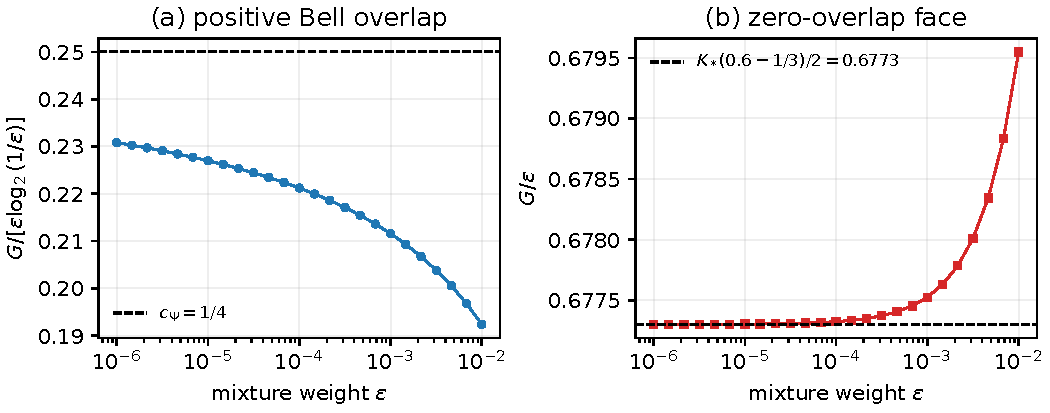
\includegraphics[width=\columnwidth]{figures/two_regime_scaling.pdf}
 \caption{Representative convergence of the capacity gap $G=K_*\chi-\CE$.  (a) For a pure-replacement perturbation, $G/[\eps\log_2(1/\eps)]$ approaches $c_\Psi=1/4$.  (b) On the zero-overlap face with $Q=\operatorname{diag}(0.6,0.3,0.1)$, $G/\eps$ approaches $K_*(0.6-1/3)/2=0.677301\ldots$.  Points are generated by the supplied script and recorded in its CSV output.}
 \label{fig:scaling}
\end{figure}

The distinction has a simple spectral origin.  At $\D$, the reference--output state for the optimal input has rank three, whereas every one-system output is full rank.  A direction with $c_\Psi>0$ populates the missing Bell component at first order, increasing the joint entropy by $c_\Psi\eps\log_2(1/\eps)$ and thereby reducing the assisted mutual information.  The ordinary output entropies have no corresponding boundary singularity.  When $c_\Psi=0$, EB geometry forces the perturbation to remain on a unital rank-deficient face; anisotropy then changes the ordinary capacity linearly while the assisted capacity is stationary to first order.

The endpoint values used in the diagnostics are
\begin{equation}
 \chi(\D)=0.081704165945510,\qquad
 \CE(\D)=0.415037499278844
 \label{eq:numericendpoint}
\end{equation}
bits per use.  They follow directly from Eq.~\eqref{eq:endpoint} and reproduce the published reverse-depolarizing benchmark.\cite{Holevo2002}

\section{Scope and conclusion}
\label{sec:conclusion}

Every fixed, nonconstant EB ray leaving the reverse-depolarizing endpoint has a strict local loss in the entanglement-assistance enhancement factor.  Generic, and in particular every nonunital, fixed direction has a nonanalytic $\eps\log(1/\eps)$ deficit whose coefficient is the Bell overlap $c_\Psi$.  The exceptional zero-overlap directions are unital and have an explicit linear deficit controlled by $q_{\max}-1/3$.

This directional stability does not imply stability on a common ball.  The lower bound $c_\Psi\geq\|\bm t_\Psi\|^2/8$ allows $c_\Psi$ to approach zero, and the constants hidden in the perturbation expansion need not be uniform as $\Psi$ changes.  A sequence of directions $\Psi(\eps)$ approaching the zero-overlap face therefore requires a genuinely two-parameter estimate.  Without such control, the sharp comparison over all qubit EB channels remains unresolved.  The present result identifies the kernel-lifting mechanism and the exceptional face that any uniform argument must treat together.

\section*{Data and code availability}

No external dataset is used.  The numerical values plotted in Fig.~\ref{fig:scaling} are generated deterministically by the supplied Python script \texttt{make\_figure.py}; its CSV output, dependency versions, and regeneration instructions accompany the manuscript.  The analytical result does not depend on the floating-point diagnostics.

\section*{Methods and generative-AI assistance}

OpenAI Codex with the GPT-5.6 Sol model (OpenAI; accessed September 2026; service build identifier not exposed) was used to accelerate structured hypothesis testing and documentation.  It assisted with exploratory algebra, deterministic diagnostic-code development, literature triage, a separate computational replay, and manuscript drafting.  It is not an author and is not used at run time to generate the numerical data or figure.  The named author must independently check the derivations, citations, originality, and final wording before submission and remains responsible for the submitted work.

\bibliographystyle{aipnum4-2}
\bibliography{references}

\end{document}
